\documentclass[12pt]{article}

%margins
\usepackage[a4paper,
inner = 25mm,
outer = 25mm,
top = 25mm,
bottom = 25mm]{geometry}

\usepackage{lmodern}
\usepackage[magyar]{babel}
\usepackage[utf8]{inputenc}
\usepackage[T1]{fontenc}
\usepackage{graphicx} %elte logo
\usepackage{amssymb}
\usepackage{amsmath} % \text{}, \substack{} in math mode
\usepackage{setspace} %spacing
\usepackage{enumerate} %enum as a)b)c)
\usepackage{nameref} %referencing chapters with names
\usepackage{tikz} %set drawings
\usepackage{proof} %unless proofs


\usetikzlibrary{arrows, calc, fit, positioning, shapes}

\definecolor{myblue}{RGB}{56, 94, 141}
\definecolor{mygreen}{RGB}{60, 179, 113}
\definecolor{myred}{RGB}{220, 20, 60}

\newcommand{\lfsih}[1] {$\lceil lf(S,#1) \rceil$}
\newcommand{\sut}{$s \subseteq A \times A^{**}$ }
\newcommand{\sprog}{$S = (s_0, \{s_1, s_2, \dots, s_n\})$ }
\newcommand{\haromszog}[2]{$#1 \vartriangleright_S #2$}
\newcommand{\egyenesnyil}[2]{$#1 \mapsto_S #2$}
\newcommand{\gorbenyil}[2]{$#1 \hookrightarrow_S #2$}


\setstretch{1.2}
\begin{document}
	
	
	\begin{titlepage}
		\vspace*{0cm}
		\centering
		\begin{tabular}{cp{1cm}c}
			\begin{minipage}{4cm}
				\vspace{0pt}
				
\includegraphics[width=1\textwidth]{elte_cimer}
			\end{minipage} & &
			\begin{minipage}{7cm}
				\vspace{0pt}Eötvös Loránd Tudományegyetem \vspace{10pt} \newline
				Informatikai Kar \vspace{10pt} \newline
				Programozási Nyelvek és Fordítóprogramok Tanszék
			\end{minipage}
		\end{tabular}
		
		\vspace*{0.2cm}
		\rule{\textwidth}{1pt}
		
		\vspace*{3cm}
		{\Huge Osztott rendszerek szintézise }
		
		\vspace*{0.5cm}
		{\normalsize IPM-08sztORSZE}
		
		\vspace{2cm}
		{\huge Konzultációs segédanyag}
		
		\vspace*{5cm}
		
		{\large \verb|Kopácsi László, Szabó Miklós|}
		
		\vfill
		
		\vspace*{1cm}
		Utolsó módosítás: \today
	\end{titlepage}
	
	\tableofcontents
	\newpage
	
	\section{konzultáció}
		\subsection{Áttekintés}
		\paragraph{}
		Az előadás során több, temporális logikai relációval találkoztunk, nézzük ezeket át informálisan, kezdve a biztonsági tulajdonságokkal.
		
	\begin{itemize}
		\item 
		Az első, melyet ''háromszög''-ként említünk ($ \vartriangleright $), bizonyos állapot-átmeneteket megenged, másokat pedig megtilt. A $(P \vartriangleright Q)$ azt jelenti, hogy a $P$ állapotot \textbf{ha} elhagyjuk, akkor ezt csak a $Q$-n keresztül tehetjük meg. A háromszög azonban nem tesz semmiféle kikötést arról, hogy a $P$-t el kell hagynunk, csupán biztosít minket arról, hogy ha ez mégis megtörténik, akkor milyen irányba (nem) mozdulhatunk.
		
		\item Másik biztonsági tulajdonság az \textit{invariáns}. Ha egy $K$ állítás invariáns, akkor ennek minden állapot-átmenet előtt és után teljesülnie kell.
		
		\item A harmadik említett kikötés a \textit{fixpont}. Ezzel leírhatjuk, hogy ha egy rendszerben már nem figyelhetünk meg további állapot-átmeneteket, akkor milyen tulajdonságoknak kell teljesülnie. $(FP \Rightarrow R)$ estén például egy $R$-el jelölt állítás igaz, amennyiben fixpontba jutottunk. Fixpontba azonban nem csak a kívánt befejezési állapot tartozhat, ha holtpont helyzet alakul ki, azt is tekinthetjük fixpontnak.
	\end{itemize}
	Természetesen nem csak biztonsági tulajdonságokra van szükségünk - azaz mit (ne) csinálhasson a rendszer -, hanem haladásira is (azért csináljon valamit).
	
	\begin{itemize}
		\item Az ''egyenes nyíl'' ($\mapsto$) néven nevezett reláció egy szigorú kikötés arra vonatkozóan, hogy egy állapotból milyen másik helyzetbe \textbf{kell} lépnünk. Míg $\vartriangleright$ esetén csupán azt mondtuk, hogy \textit{ha} elhagyunk egy állapotot, akkor azt milyen irányba tegyük, a $(P \mapsto Q)$ azt mondja, hogy a $P$ állapotból a $Q$ állapotba kell, hogy kerüljünk (véges időn belül).
		\item Ennél megengedőbb a ''görbe nyíl''-ként ($\hookrightarrow$) ismert reláció. Ebben az esetben a $(A \hookrightarrow B)$ feltétel csupán annyit mond, hogy az $A$ állapotot előbb-utóbb a $B$ állapot fogja követni (azaz $A$-ból elkerülhetetlenül $B$-be fogunk érkezni), de itt nincs semmilyen megkötés arra, hogy a két állapot egymás után következzen be. Legális állapot-átmenet sorozat az $(A \hookrightarrow B)$-ra az $<A, G, F, D, F, E, C, D, B>$ is.
	\end{itemize}

\subsection{Étkező filozófusok}\label{etkezo-filo}
	Tekintsük az előadáson is ismertetett \textit{étkező filozófusok} feladatot (jegyzet\textsuperscript{\cite{orsi_jegyzet}} 1.1). Próbáljuk meg kiegészíteni a feltételeket további megkötések formalizálásával:
	\begin{itemize}
		\item Ha a rendszer nyugalmi állapotban van, akkor egy filozófus sem eszik.
		\item Mindegyik filozófusra igaz, hogy ha hazament, akkor utána már nem kerülhet más állapotba.
	\end{itemize}

\subsection{Moziterem}\label{moziterem-feladat}
	A következő példában egy mozira vonatkozó feladatot fogunk ismertetni, ahol a nézők tevékenységére szeretnénk megkötéseket tenni. A jelölést megkönnyítendő vezessük be az alábbiakat: $n(i)$ jelölje az $i$-ik nézőt. A moziba látogatók állapotait az alábbiak alapján jelöljük:
	\begin{enumerate}[a)]
		\item megérkezik a moziba - a
		\item jegyet vesz - j
		\item üdítőt és nasit vásárol - b
		\item érvényes jeggyel rendelkezik - t
		\item filmet néz - f
		\item hazamegy - h
	\end{enumerate}
	Próbáljuk formalizálni az alábbi feltételeket:
	\begin{itemize}
		\item A moziba érkező néző filmet fog nézni.
		\item Ha valaki érvényes jeggyel rendelkezik, akkor megnézi a filmet.
		\item Ha a moziban nincs mozgás, akkor minden néző már otthon van.
		\item A moziba érkező néző jegyet vásárol, vagy a büfébe megy.
		\item A film után a néző hazamegy.
		\item Senki nem nézhet filmet úgy, hogy nincs érvényes jegye. (Tipp: próbáljunk invariánst megfogalmazni.)
		\item Ha valaki hazament, akkor már nem csinál semmit a moziban.
	\end{itemize}

\newpage
\section{konzultáció}
\subsection{Áttekintés}
Ahhoz, hogy a későbbiekben biztos módon számolhassunk programokkal , elkerülhetetlen a számunkra szükséges (alap)fogalmakat tisztázni a halmazelmélet és a relációk témakörében.

Legyenek $A$ és $B$ tetszőleges halmazok. $A$ és $B$ \textit{direkt-}, vagy \textit{Descartes}-szorzatán azt a halmazt értjük, melyben olyan párok találhatóak, melynek első eleme $A$-, második eleme pedig $B$-beli.
$$A \times B ::= \{ (a,b) | a \in A \text{ és } b \in B \}$$
Jelölje $r \subseteq A \times B$ azt a bináris relációt, mely $A$ elemeihez rendel értékeket a $B$ halmazból ($A$ és $B$ tetszőleges halmazok). A reláció elemeit $(a,b) \in r $ módon fogjuk jelölni.
$$ \text{Az } r \text{ reláció értelmezési tartománya: } \mathcal{D}_r ::= \{a \in A | \exists b \in B: (a,b) \in r \} \subseteq A$$
$$ \text{Az } r \text{ reláció értékkészlete: } \mathcal{R}_r ::= \{b \in B | \exists a \in A: (a,b) \in r \} \subseteq B$$
$$\ r(a) \text{ jelölje azt a halmazt, melynek elemei: } \{b \in B | (a,b) \in r \} $$

Világos, hogy az értelmezési tartományban olyan elemek vannak, amikhez rendel valamit $r$, míg az értékkészletben olyanokat találhatunk, amik valamilyen elemhez hozzá lettek rendelve. Egy elem képe a hozzá rendelt elemek halmazából áll elő.

Egy $g$ relációt \textit{parciális függvény}nek (vagy determinisztikus relációnak) nevezhetünk, amennyiben az alábbi teljesül:
$$\forall a \in A : |g(a)| \le 1,$$ azaz minden elemhez \textit{legfeljebb} egy másikat társítunk.
Jelölésünk ekkor: $g \in A \rightarrow B$.
Ha minden elemhez pontosan egy értéket rendelünk, akkor az $f$ reláció függvény, azaz:
$$\forall a \in A : |f(a)| = 1. $$
Jelölésünk ekkor: $ f: A \rightarrow B $. Ebben az esetben általában $f(a)$ nem az egy elemű halmazt, hanem annak képét jelenti.

Ahhoz, hogy állításokat fogalmazhassunk meg a későbbiekben, szükségünk lesz logikai relációkra is.
$$\text{A } h \subseteq A \times \mathbb{L} \text{ logikai relációnak nevezzük, ahol } \mathbb{L} ::= \{igaz, hamis\}.$$
Ha $h$ függvény, akkor \textit{logikai függvény}nek nevezzük.\\
Egy reláció inverzét az alábbi módon definiálhatjuk:
$$R^{(-1)} ::= \{(b,a) \in B \times A | (a,b) \in R  \}$$

A továbbiakban szükségünk lesz egy reláció adott halmazra vonatkozó inverz- és őskép definíciójára.\\
A $H \subseteq B $ halmaz $R$ reláció szerinti \textit{inverz}képe:
$$ R^{(-1)}(H) ::= \{ a \in A | R(a) \cap H \ne \varnothing \}$$
A $H \subseteq B $ halmaz $R$ reláció szerinti \textit{ős}képe:
$$ R^{-1}(H) ::= \{ a \in A | R(a) \subseteq H \}$$

Meggondolva látható, hogy az \textit{inverzkép} megengedőbb, hisz csak annyit kér, hogy egy adott elemhez \textit{létezzen} $H$-beli elem az $R$ hozzárendelésben, az \textit{őskép} viszont megköveteli, hogy \textit{minden} ilyen elem a $H$ halmazban legyen.

\begin{figure}[!ht]
	\centering
	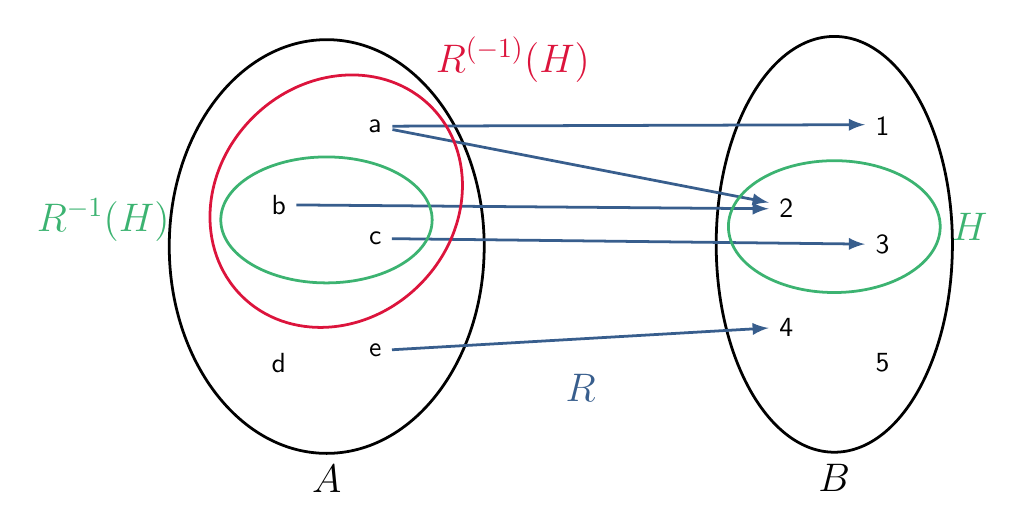
\begin{tikzpicture}[line width=1pt,>=latex]
	\sffamily
	\node (a1) {a};
	\node[below=of a1] (a3) {c};
	\node[left=of $(a1)!0.7!(a3)$] (a2) {b};
	\node[below=1.5cm of a2] (a4) {d};
	\node[below=of a3] (a5) {e};
	
	\node[right=6cm of a1] (b1) {1};
	\node[below=of b1] (b3) {3};
	\node[left=of $(b1)!0.7!(b3)$] (b2) {2};
	\node[below=of b2] (b4) {4};
	\node[below=of b3] (b5) {5};
	
	\node[shape=ellipse, draw=black, minimum size=4cm, fit={(a1) (a2) (a4) (a5)}] (A) {};
	\node[shape=ellipse, draw=black, minimum size=3cm, fit={(b1) (b2) (b4) (b5)}] (B) {};
	
	\node[below=0cm of A,font=\Large\bfseries] {$A$};
	\node[below=0cm of B,font=\Large\bfseries] {$B$};
	
	
	\draw[->,myblue] (a1) -- (b1.175);
	\draw[->,myblue] (a1) -- (b2.160);
	\draw[->,myblue] (a2) -- (b2);
	\draw[->,myblue] (a3) -- (b3);
	\draw[->,myblue] (a5) -- (b4);
	
	\node[below=1.5cm of $(A)!0.5!(B)$,font=\color{myblue}\Large\bfseries] {$R$};
	
	
	\node[shape=ellipse, draw=mygreen, fit={(b2) (b3)}] (H) {};
	\node[shape=ellipse, draw=mygreen, fit={(a2) (a3)}] (Ros) {};
	\draw[rotate=-45, myred] ($(a1)!0.8!(Ros)$) ellipse (1.5cm and 1.7cm);
	
	\node[right=0cm of H,font=\color{mygreen}\Large\bfseries] {$H$};
	\node[left=0.5cm of Ros,font=\color{mygreen}\Large\bfseries] {$R^{-1}(H)$};
	\node[above=0.5cm of a1] (align1) {};
	\node[right=0.5cm of align1,font=\color{myred}\Large\bfseries] {$R^{(-1)}(H)$};
	
	\end{tikzpicture}
	\caption{Nézzünk egy példát a korábban említett fogalmakra. Legyen $A=\{a, b, c, d, e\}$ és $B=\{1, 2, 3, 4, 5\}$ halmazok, valamint $R \subseteq A \times B, R=\{(a,1), (a,2), (b, 2), (c, 3), (e, 4)\}$ reláció. Ekkor $R$ \textit{értelmezési tartománya} $\mathcal{D}_R=\{a, b, c, e\}$, \textit{értékkészlete} pedig $\mathcal{R}_R=\{1,2,3,4\}$. Továbbá legyen $H \subseteq B, H=\{2, 3\}$. Ekkor a $H$ halmaz $R$ reláció szerinti \textit{ősképe} $R^{-1}(H)=\{b, c\}$,  \textit{inverzképe} pedig $R^{(-1)}(H)=\{a,b,c\}$. Itt jól látszik, hogy az \textit{inverzkép} megengedőbb, mint az \textit{őskép}, hiszen $R^{-1}(H) \subseteq R^{(-1)}(H) = \{b, c\} \subseteq \{a,b,c\}$.}
	\label{fig:halmazok}
\end{figure}

Legyen $R \subseteq A \times \mathbb{L}$ logikai reláció, $R$ igazsághalmaza ekkor:
$$  \lceil R \rceil ::= R^{-1}(\{igaz\}) \text{ azaz: } \lceil R \rceil = \{a \in \mathcal{D}_R | R(a) \subseteq \{igaz\} \} $$
Az igazsághalmazt tehát az $\{igaz\}$ halmazra vett őskép szerint definiáljuk.\\
Ha inverzképet számolunk, akkor juthatunk a \textit{gyenge igazsághalmaz} fogalmához:
$$  \lfloor R \rfloor ::= R^{(-1)}(\{igaz\}) \text{ azaz: } \lfloor R \rfloor = \{a \in \mathcal{D}_R | R(a) \cap \{igaz\} \ne \varnothing \} $$

A későbbiekben nagyban megkönnyíti a dolgunkat, ha bevezetjük az \textit{azonosan igaz}, és az \textit{azonosan hamis} logikai függvényeket.
$$Igaz: A \rightarrow \mathbb{L}: \forall a \in A: Igaz(a) = \{igaz\} $$
$$Hamis: A \rightarrow \mathbb{L}: \forall a \in A: Hamis(a) = \{hamis\} $$
Könnyű meggondolni, hogy ekkor $\lceil Igaz \rceil = A \text{ és } \lceil Hamis \rceil = \varnothing $.\\
Az igazsághalmazzal kapcsolatban fontos megemlíteni néhány tulajdonságot, melyeket a későbbiekben kihasználunk.\\
\\
Legyenek $P$, $Q \subseteq A \times \mathbb{L}$, ekkor:
\begin{itemize}
	\item $ \lceil P \land Q \rceil = \lceil P \rceil \cap \lceil Q \rceil $
	\item $ \lceil P \lor Q \rceil = \lceil P \rceil \cup \lceil Q \rceil  $
	\item $	\lceil \neg P \rceil = A \setminus \lceil P \rceil  $
	\item $\lceil P \rightarrow Q \rceil = \lceil \neg P \lor Q \rceil = (A \setminus \lceil P \rceil) \cup \lceil Q \rceil $
	\item $ P \Rightarrow Q = \lceil P \rceil \subseteq \lceil Q \rceil $
\end{itemize}

Egyszerűbben megfogalmazhatóak állítások, ha tudjuk, hogy $A \Rightarrow B$. Ekkor ugyanis:
\begin{itemize}
	\item $A \lor B = B$
	\item $A \land B = A$
\end{itemize}
Nézzünk erre egy példát, legyenek $A$, $B: \mathbb{N} \times \mathbb{L}$ úgy, hogy:\\
$\lceil A \rceil := $\{10-nél nagyobb szám\} és\\
$\lceil B \rceil := $ \{pozitív szám\}.\\
Világos, hogy $A \Rightarrow B$, hiszen ha egy egész szám 10-nél nagyobb, akkor pozitív.
Az $A \lor B$ állítást úgy fogalmazhatjuk meg, hogy azokat az egész számokat keressük, melyek 10-nél nagyobbak, \textbf{vagy} pozitívak. Érződik, hogy a \textit{vagy} kapcsolat miatt a gyengébb feltétellel is megelégszünk, így a bővebb halmaz, azaz a pozitív számok halmazát kapjuk $(=B)$. Ha azonban a 10-nél nagyobb \textbf{és} pozitív számokra vagyunk kíváncsiak, akkor a szigorítás miatt a szűkebb halmazt kapjuk, tehát a 10-nél nagyobb számokat kell vizsgálnunk $(=A)$.

\subsection{Program}

Röviden tekintsük át, hogy a Fóthi\textsuperscript{\cite{fothi_biblia}}-Horváth - féle modellben hogyan is definiáltuk a programot és annak hatásrelációját.

Jelölje $A^*$ az $A$ elemeiből képzett véges, $A^\infty$ pedig a végtelen sorozatokat. A későbbiekben $A^{**}$ jelenti az $A^* \cup A^{\infty}$ halmazt, azaz a véges és végtelen sorozatok halmazát. Ha alaphalmaznak a természetes számokat választjuk, akkor az $<1, 5, 3, 2> \in A^*$ egy véges, míg az $<1, 2, 3, 4, ...> \in A^{\infty}$ végtelen sorozatot jelöl.\\

\textit{Utasítás} alatt egy olyan \sut relációt értünk, melyre:
\begin{enumerate}
	\item $\mathcal{D}_s = A$
	\item $\forall a \in A : \forall \alpha \in s(a) : |\alpha|\ne 0 \land  \alpha_1 = a $
	\item $(\alpha \in \mathcal{R}_s \land \alpha \in A^*  ) \Rightarrow (\forall i (1 \le i < |\alpha|): \alpha_i \ne \alpha_{i+1} )$
	\item $(\alpha \in \mathcal{R}_s \land \alpha \in A^{\infty}) \Rightarrow (\forall i \in \mathbb{N}: (\alpha_{i} = \alpha_{i+1} \rightarrow (\forall k \in \mathbb{N^+}: \alpha_{i} = \alpha_{i+k}))$
\end{enumerate}
A fenti definíció a \textit{működés} fogalmát próbálja absztrakt módon szemléltetni. A négy pont jól jellemzi az utasítást: elsőként szeretnénk, ha az utasítás minden állapottér-beli pontban értelmezve lenne (azaz az utasítás mindenhonnan el tud indulni).\\
Második pontban azt fogalmazzuk meg, hogy egy sorozat a működése teljes történetét írja le, kezdve a kiindulási állapottal.\\
A harmadik pontunk a \textit{redukáltságra} vonatkozik: ha véges hosszú sorozattal dolgozunk, akkor egymás után kétszer ne szerepelhessen ugyanaz az elem (hiszen az nem egy jó véges utasítás, amelyik úgy lép egy következő állapotba, hogy nem történt állapotváltozás - ez a megfogalmazáson is érződik).\\
A negyedik pont a végtelen utasításra utal: ha egy utasítás futása nem fejeződik be (végtelen ciklus, stb.), akkor ezt a hozzárendelt sorozatban úgy jelzi, hogy egy adott ponttól kezdve nem történik állapotváltozás, folyton ugyan abban az állapotban ragad (pl. $s(4) = <4, 3, 2, 1, 0, 0, 0, 0, 0, 0, ...>$) \\


Egy \sut utasítás \textit{hatásreláció}ja az a $p(s) \subseteq A \times A$ reláció, melyre:
\begin{enumerate}
	\item $ \mathcal{D}_{p(s)} = \{a \in A | s(a) \subseteq A^* \} $
	\item $ p(s)(a) = \{ b \in  A | \exists \alpha \in s(a) : \tau(\alpha) = b  \}$
\end{enumerate}
ahol $\tau: A^* \rightarrow A; \tau(\alpha) ::= \alpha_{|\alpha|}$, azaz a \textit{tau} függvény egy véges sorozathoz annak utolsó tagját rendeli.

A hatásrelációt tehát csak olyan pontokban definiáljuk, ahol a program \textit{megáll}, azaz véges sorozatot rendel, a hozzárendelési szabály pedig az, ahová az utasítás eljut, tehát az adott sorozatok utolsó eleme.


Az \textit{absztrakt program}ot egy \sprog párként tudjuk megadni, ami egy párhuzamos programot takar. Az első tagja ($s_0$) a kezdeti utasítás, ami a program indulásakor hajtódik végre. A második tagja ($\{s_1, s_2, \dots, s_n\}$) pedig \textit{atomi} (vagyis párhuzamos futás során nem akadnak össze, szekvenciális futás eredményét adó) utasítások halmaza. Ezeket valamilyen \textit{feltétlenül pártatlan ütemezés} szerint (kiéheztetés nélkül, azaz az egyes végrehajtások során minden utasítást végtelen sokszor véve) végtelen sokáig futtatunk. A programra pedig akkor mondjuk, hogy terminált (befejeződött), ha fixpontba jut, azaz már nem történik állapotváltozás.

Nézzünk erre egy egyszerű példát:\\
Legyen $S = (x := 0, \{x := 2 \cdot x, x := x + 1\})$. Ekkor az alábbi sorozatot ennek egy lehetséges kiértékelésének tekintjük:
\begin{align*}
	x &:= 0,	&x &:= x + 1,	&x &:= 2*x,	&x &:= 2*x,	&x &:= x + 1,	&x &:= x + 1,	&&\dots\\
	&0,	&&1,	&&2,	&&4, &&5,	&&6,	&&\dots
\end{align*}


\subsection{Leggyengébb előfeltétel}
Érezhető, hogy a fenti definíciókkal történő számolások nagyon nehézzé fogják tenni a későbbiekben a feladatok és az azt megoldó programok közötti kapcsolat megteremtését, ezért bevezetünk egy új fogalmat, a \textit{leggyengébb előfeltétel}t.

\paragraph{}
Legyen \sut utasítás, $R: A \rightarrow \mathbb{L}$ állítás. Az $s$ utasítás $R$ utófeltételhez tartozó \textit{leggyengébb előfeltétele} az az $lf(s,R): A \rightarrow \mathbb{L}$ \textbf{függvény}, melyre:
$$ \lceil lf(s,R) \rceil = \{ a \in \mathcal{D}_{p(s)} | p(s)(a) \subseteq \lceil R \rceil \}. $$
\par Az \textit{lf} tehát egy olyan függvény, mely pontosan azokhoz a pontokhoz rendel igazat, melyből elindítva az $s$ utasítást az biztosan megáll, és az összes ilyen állapotban az $R$ tulajdonság teljesül.
Magának a függvénynek a definícióját legtöbbször nehéz megadni, de az igazsághalmazát könnyedén kifejezhetjük. Az igazsághalmaz definícióját, a kompozíció és az őskép tulajdonságait felhasználva kapjuk, hogy:
$$\lceil lf(s,R)\rceil = \lceil R \circ p(s) \rceil.$$
Az \textit{lf}-et tehát az utófeltételbe helyettesítés módszerével tudjuk kifejezni (ennek bizonyítása megtalálható a \textit{tankönyv}\textsuperscript{\cite{fothi_biblia}} 44-ik oldalán, a 3.1-es definíciónál). 

\par Mivel a leggyengébb előfeltételt nem csak utasításokra, hanem programokra is ki szeretnénk tudni számolni, a fenti definíciót picit általánosítani kell. Tehát legyen \sprog program, $R: A \rightarrow \mathbb{L}$ állítás. Ekkor az $S$ program $R$ utófeltélhez tartozó \textit{leggyengébb előfeltétele} az egyes utasításai által adott leggyengébb előfeltételek konjugáltja lesz:
$$ lf(S, R) = \bigwedge_{i=1}^n lf(s_i, R). $$


A későbbiekben több alaptulajdonságra is szükségünk lesz, ha az \textit{lf}-fel akarunk számolni. Nézzük ezeket:
\paragraph{}
Legyen \sprog program, $Q,R: A \rightarrow \mathbb{L}$ állítások. Ekkor:
\begin{enumerate}
	\item $lf(S, Hamis) = Hamis$ (csoda kizárásának elve),
	\item Ha $Q \Rightarrow R$, akkor $lf(S,Q) \Rightarrow lf(S,R)$ (monotonitás),
	\item $lf(S,Q) \lor lf(S,R) \Rightarrow lf(S, Q\lor R)$ (gyenge additivitás),
	\item $lf(S,Q) \land lf(S,R) = lf(S, Q\land R)$ (multiplikativitás)
\end{enumerate}
A bizonyításokat szintén a jegyzetben lehet olvasni.

\begin{figure}[!ht]
	\centering
	\begin{tikzpicture}[line width=1pt,>=latex]
	
	%balhalmaz
	\sffamily
	\node (a1) {a};
	\node[below=of a1] (a3) {c};
	\node[left=of $(a1)!0.7!(a3)$] (a2) {b};
	\node[below=1.5cm of a2] (a4) {d};
	\node[below=of a3] (a5) {e};
	
	%jobboldali halmaz elemei
	\node[right=6cm of a1] (b1) {e};
	\node[below=of b1] (b3) {b};
	\node[left=of $(b1)!0.7!(b3)$] (b2) {a};
	\node[below=of b2] (b4) {c};
	\node[below=of b3] (b5) {d};
	
	\node[shape=ellipse, draw=black, minimum size=3.5cm, fit={(a1) (a2) (a4) (a5)}] (A) {};
	\node[shape=ellipse, draw=black, minimum size=3.5cm, fit={(b1) (b2) (b4) (b5)}] (A2) {};
	
	%halmazcimke
	\node[below=0cm of A,font=\Large\bfseries] {$A$};
	\node[below=0cm of A2,font=\Large\bfseries] {$A$};
	
	
	%hozzárendelések a két halmaz között
	\draw[->,myblue] (a1) -- (b1.175);
	\draw[->,myblue] (a1) -- (b2.160);
	\draw[->,myblue] (a2) -- (b2);
	\draw[->,myblue] (a3) -- (b3);
	\draw[->,myblue] (a5) -- (b4);
	
	%nyílra írt szöveg
	\node[below=1.5cm of $(A)!0.5!(B)$,font=\color{myblue}\Large\bfseries] {$p(s)$};
	
	
	\node[shape=ellipse, draw=mygreen, fit={(a2) (a3)}] (LfsRih) {};
	\node[shape=ellipse, draw=myred, fit={(b2) (b3)}] (Rih) {};
	
	%lf(s,R) ih.
	\node[left=0.5cm of LfsRih,font=\color{mygreen}\Large\bfseries] { \lfsih{R} };	
	%R ih
	\node[right=0.5cm of Rih,font=\color{myred}\Large\bfseries] {$\lceil R \rceil$};
	
	
	\end{tikzpicture}
	\caption{Legyen $A = \{a,b,c,d,e\}$ halmaz és $p(s) := \{(a,a), (a,e), (b,a), (c,b), (e,c) \} $ hatásreláció, $\lceil R \rceil = \{a,b\}$. $lf(s,R)$ ekkor azokban a pontokban lesz igaz, melyben $p(s)$ értelmezve van és minden ezekhez rendelt elem $R$ igazsághalmazában található. Végiggondolva tehát \lfsih{R} ekkor $=\{b,c\}$.}
	\label{fig:lfsrzemleltetes}
\end{figure}

\paragraph{Kiszámítása:}
Az \textit{lf} kiszámolását a már fentebb említett utófeltételbe helyettesítés módszerével tudjuk megtenni.

Az \textbf{egyszerű értékadás}ok során ez a következőt jelenti:
$$lf(x := y, R) = R^{x \leftarrow y } $$
Például az $s = (x := 3), R = (1 \le x \le 5)$ esetben:\\
$lf(s, R) = lf(x:=3, (1 \le x \le 5)) = R^{x \leftarrow y} = (1 \le x \le 5)^{x \leftarrow 3} = (1 \le 3 \le 5)$.
Az $s$ utasítás tehát olyan állapotokban tudjuk biztonságosan végrehajtani úgy, hogy $R$-be érkezzen, melyre teljesül az, hogy $1 \le 3 \le 5 \equiv igaz$, azaz tetszőleges pontból indítva helyesen működő utasítást kaphatunk.

\textbf{Feltételes értékadás} esetén figyelembe kell venni a feltételt is, hiszen ha ez nem teljesül, abban az esetben nem kell az értékadást végrehajtanunk.
$$lf(\{x:=y, \text{ha } \pi\}, R) = (\pi \rightarrow R^{x \leftarrow y}) \land (\neg \pi \rightarrow R^{SKIP})$$
Például az $s = (x := -x, ha\ x < 0), R = (x > 0)$ esetben:
\begin{align*}
	lf(s, R) = lf((x := -x, ha\ x < 0), x > 0) &= (x < 0 \rightarrow (x > 0)^{x \leftarrow -x}) \land (x \ge 0 \rightarrow x > 0)\\
	&= (x < 0 \rightarrow -x > 0) \land (x \ge 0 \rightarrow x > 0)
\end{align*}
Ekkor az $A \rightarrow B = \neg A \lor B$ logikai szabályt alkalmazva az alábbit kapjuk:
$$ (x \ge 0 \lor -x > 0) \land (x < 0 \lor x > 0) = (x \ge 0 \lor x < 0) \land (x \neq 0) = (\uparrow) \land (x \neq 0) = (x \neq 0)$$
Vagyis az $s$ utasítást minden $x \neq 0$ állapotban biztonságosan végre tudjuk hajtani úgy, hogy $R$-be érkezzen.

\textbf{Szimultán értékadás} során egyszerre hajtjuk végre az adott értékadásokat:
$$lf(\{x_1, ..., x_n := y_1, ..., y_n\}, R) = lf(\{ \mathop{\parallel}_{i=1}^{n} x_i := y_i \}, R) = R^{\substack{ x_1 \leftarrow y_1 \\ ... \\ x_n \leftarrow y_n }}$$
Például az $s = (x,y := x + 1, y - 1), R = (2 | x + y)$ esetben:
\begin{align*}
	lf(s, R) &= lf((x,y := x + 1, y - 1), (2 | x + y)) \\
		&= (2 | x + y)^{\substack{ x \leftarrow x + 1 \\ y \leftarrow y - 1 }} \\
		&= (2 | (x + 1) + (y - 1)) = (2 | x + y)
\end{align*}
Azaz az $s$ utasítást olyan $x, y$ állapotokban tudjuk biztonságosan végrehajtani úgy, hogy $R$-be érkezzen, melyre teljesül az, hogy $2 | x + y$.

A \textbf{feltételes szimultán értékadás} kiszámításának módja ezek után egyértelműen megállapítható az előzőek alapján:
$$lf(\{x_1, ..., x_n := y_1, ..., y_n, \text{ha } \pi \}, R) = lf(\{ \mathop{\parallel}_{i=1}^{n} x_i := y_i, \text{ha }\pi \}, R) = $$
$$= (\pi \rightarrow R^{\substack{ x_1 \leftarrow y_1 \\ ... \\ x_n \leftarrow y_n }}) \land (\neg \pi \rightarrow R^{SKIP})$$

\subsection{Feladatok}\label{lf-feladat}
A következő példákkal a leggyengébb előfeltétel számítását tudjuk gyakorolni.

\begin{enumerate}
	\item Legyen $\begin{aligned}[t]
			S = (SKIP, \{x &:= x \cdot 2, ha\ 2 \nmid x,\\
				x &:= x + 1, ha\ x < 10\}),
		\end{aligned}$\\
		és $R = (2 | x)$. Számoljuk ki az $S$ program $R$-hez tartozó leggyengébb előfeltételét.
	\item Legyen $\begin{aligned}[t]
			S = (m,n := 0,0,\ \{m,n &:= m+1, n-1,\\
				n &:= n + 1, ha\ n < m\}).
		\end{aligned}$\\
		Számoljuk ki az $S$ program $R$-hez tartozó leggyengébb előfeltételét.
		\begin{enumerate}[a)]
			\item Ha $R = (m = n).$
			\item Ha $R = (n > m).$
		\end{enumerate}
\end{enumerate}


\section{konzultáció}
\subsection{Gyakorlás}
\paragraph{}Először gyakoroljunk pár további \textit{lf} számolást.\\
\begin{enumerate}
	\item  Legyen $\begin{aligned}[t]
			s &= \{x := -x, \text{ha } x>0\}, \text{ és}\\
			R &= (x>1).\\
			lf(s,R) &= ? \\
			 \\
			\lceil lf(s,R) \rceil &= (x>0 \rightarrow (x>1)^{x \leftarrow -x}) \land (x \le 0 \rightarrow x > 1) \\
			&= (x>0 \rightarrow -x>1 ) \land (x \le 0 \rightarrow x > 1) \\
			&= (x \le 0 \lor -x > 1) \land (x > 0 \lor x > 1) \\
			&= (x \le 0 \lor x < 1) \land (x>0) \\
			&= (x \le 0) \land (x>0) \equiv Hamis.
			\end{aligned}$\\
		Átgondolva mit is akartunk kiszámolni, milyen állapotból indulva teljesíthető az a követelmény, hogy $(x>1)$, ha a programunk a pozitív számokon előjelet vált, a negatívakat (és nullát) pedig nem változtatja?\\
		Ha pozitív bemenetet kap, akkor negatívat csinál belőle, negatívakra pedig nem csinál semmit, tehát sehogy sem tudjuk elérni, hogy tetszőleges bemenetre elérjünk a kívánt állapotba, ezért az azonosan $Hamis$ az eredmény.
	\item Legyen $\begin{aligned}[t]
	S = (SKIP, \{x&:=0, \text{ ha } y \ne 0, \\
				x&:=x*z, \text{ ha } z = 0\})\\
				R &= (x=0)\\
	lf(S,R) &= ? \dots \#magic\\
	lf(S,R) &= (x=0) \lor (y \ne 0 \land z=0)\\
	%TODO megoldást beírni.
	\end{aligned}$\\
\end{enumerate}

\subsection{Stabilitási tulajdonság}
Biztonsági tulajdonságot már néztünk a feladatok kapcsán, ám utasításokra (és programokra) is szeretnénk ilyet definiálni.
$$\text{Legyenek }P,Q: A \rightarrow \mathbb{L} \text{ állítások, és } s \subseteq A \times A^{**} \text{ utasítás.}$$
$$P \vartriangleright_s Q ::= (P \land \neg Q) \Rightarrow lf(s, P \lor Q)$$
A $P$ állapotot az utasítás ekkor \textit{ha} elhagyja, akkor ezt csak $Q$-n keresztül teheti meg.

\begin{figure}[!ht]
	\centering
	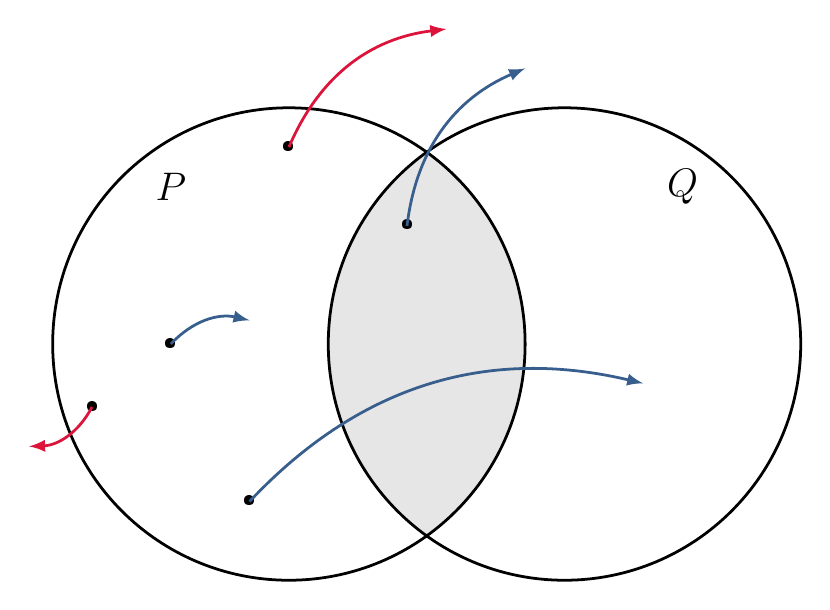
\begin{tikzpicture}[line width=1pt,>=latex]
	
	% define sets
	\def\firstset{(3,3) ellipse (3 and 3)}
	\def\secondset{(6.5,3) ellipse (3 and 3)}		
	
	% color sets
	% \fill[mygreen] \firstset \secondset;
	
	% color intersection
	\begin{scope}
	\clip \firstset;
	\fill[gray, opacity=0.2] \secondset;
	\end{scope}
	
	% outline of sets
	\draw \firstset \secondset;
	
	% set labels
	\node[font=\Large\bfseries] at (1.5,5) {$P$};
	\node[font=\Large\bfseries] at (8,5) {$Q$};
	
	% Nope points/arrows
	\foreach \ax/\ay/\bx/\by in {
		3/5.5/5/7,
		0.5/2.2/-0.3/1.7
	}{
		\node at (\ax, \ay) {\textbullet};
		\path[->, myred] (\ax, \ay) edge [bend left] (\bx, \by);
	}
	
	% Correct points/arrows
	\foreach \ax/\ay/\bx/\by in {
		4.5/4.5/6/6.5,
		1.5/3/2.5/3.3,
		2.5/1/7.5/2.5
	}{
		\node at (\ax, \ay) {\textbullet};
		\path[->, myblue] (\ax, \ay) edge [bend left] (\bx, \by);
	}
	
	
	\end{tikzpicture}
	\caption{Nézzünk egy szemléletesebb példát a háromszög tulajdonságra. $P \vartriangleright_s Q$ akkor és csak akkor teljesül, ha $(P \land \neg Q)$-ból bárhogy választunk állapotokat, az $s$ utasítás hatására ugyanúgy $(P \land \neg Q)$-ban maradunk, vagy pedig $Q$-ba jutunk. Jó átmeneteknek számítanak a kék nyilak, viszont a piros nyilakról ez nem mondható el.}
	\label{fig:haromszog}
\end{figure}


A \textit{háromszögre} fontos néhány tulajdonságot megjegyezni, melyet a definíció alapján igazolhatunk.


\begin{itemize}
	\item $P \vartriangleright_s P = P \land \neg P \Rightarrow lf(s,P \lor P) = \downarrow \Rightarrow lf(s,P) = \uparrow \lor lf(s,P) = \uparrow$
	\item $P \vartriangleright_s \neg P = P \land P \Rightarrow lf(s,P \lor \neg P) = P \Rightarrow lf(s,Igaz) = \uparrow$
	\item $Igaz \vartriangleright_s P = Igaz \land \neg P \Rightarrow lf(s,Igaz \lor P) = \neg P \Rightarrow lf(s,Igaz) = \uparrow$
	\item $Hamis \vartriangleright_s P = Hamis \land \neg P \Rightarrow lf(s, Hamis \lor P) = Hamis \Rightarrow lf(s,P) = \uparrow$
	\item $P \vartriangleright_s Igaz = P \land Hamis \Rightarrow lf(s,P \lor Igaz) = Hamis \Rightarrow lf(s,Igaz) = \uparrow$
	
\end{itemize}
Fontos megjegyezni, hogy általános esetben a $P \vartriangleright_s Hamis$ nem teljesül.\\
$P \vartriangleright_s Hamis = P \land Igaz \Rightarrow lf(s,P \lor Hamis) = P \Rightarrow lf(s,P)$, de erről nem tudunk tetszőleges program és állítás esetén semmit garantálni.\\
Egy példa erre, mikor nem teljesül:\\
$s = (x := x+1) \text{ és } P = (2|x) \\
P \vartriangleright_s Hamis = P \Rightarrow lf(s,P) = (2|x) \Rightarrow lf(x:=x+1, 2|x) = (2|x) \Rightarrow (2|x)^{x \leftarrow x+1} = (2|x) \Rightarrow (2|x+1) $, ami nyilvánvaló ellentmondás, hiszen ha egy szám páros, akkor a nála eggyel nagyobb szám nem lehet szintén páros (mivel az páratlan).
\paragraph{}Abban az esetben azonban, \textit{ha} $P \vartriangleright_s Hamis$ teljesül, akkor azt mondjuk, hogy $s$ rendelkezik a $P$ stabil tulajdonsággal, azaz $P$-ből nem tud kivezetni a program. Jelölésünk erre: $P stabil_s$ (triviálisan stabil tulajdonság az $Igaz$, hiszen $Igaz \Rightarrow lf(s,Igaz)$ tetszőleges utasításra teljesül).

A háromszög azonban nem tranzitív, azaz $ P \vartriangleright_s Q \text{ és } Q \vartriangleright_s R$-re általában \textbf{nem igaz}, hogy $P \vartriangleright_s R$.


\paragraph{Feladat}
\par Számoljuk ki \haromszog{P}{Q}-t, ha:\\
$
\begin{aligned}[r]
S = (SKIP, \{s_1: x :&= x+2, \text{ ha } x<50, \text{ és}\\
s_2: x :&= x+1, \text{ ha } x\ge 50 \}\\
&P = (2|x)\\
&Q = (x\ge50)\\
 \\
P \vartriangleright_S Q &= lf(S, P \lor Q)\\
(2|x)\land (x<50) &\Rightarrow lf(S, (2|x \lor x\ge50)) \\
\text{Az } lf &\text{ multiplikativitását felhasználva:}\\
lf(S,P \lor Q) &= lf(s_1, P\lor Q) \land lf(s_2, P\lor Q)\\
s1: lf(x:=x+2, \text { ha } x<50 &, (2|x \lor x\ge50) ) = \\
(x<50 &\rightarrow (2|x \lor x\ge50)^{x \leftarrow x+2}) \land \\
\land (x\ge50 &\rightarrow (2|x \lor x\ge50))\\
=(x\ge50 \lor 2|x+2 \lor x+2\ge50) = (x\ge50 \lor 2|x &\lor x\ge48)= (x\ge48 \lor 2|x)\\
s2: lf(x:=x+1, \text { ha } x\ge50 &, (2|x \lor x\ge50) ) = \\
(x\ge50 &\rightarrow (2|x \lor x\ge50)^{x \leftarrow x+1}) \land \\
\land (x<50 &\rightarrow (2|x \lor x\ge50))\\
=(x\ge50 \rightarrow 2|(x+1) \lor x+1\ge50) &\land (x<50 \rightarrow 2|x \lor x\ge50)\\
=(x<50 \lor 2|x+1 \lor x\ge49) &\land (x\ge50 \lor 2|x \lor x\ge50)\\
=(\uparrow) &\land (2|x \lor x\ge50)\\
\text{A két eredményt éselve: } lf(S,P\lor Q) &= lf(s_1,P\lor Q) \land (s_2, P \lor Q)\\
=(x\ge48 \lor 2|x) \land (x\ge50 \lor 2|x) &= 2|x \lor x\ge50\\
P\land \neg Q &\Rightarrow lf(S,P\lor Q) \text{ behelyettesítve ekkor:}\\
(2|x \land x<50) &\Rightarrow (2|x \lor x\ge50) \text{ pedig igaz }2|x\text{ miatt,}\\
\text{hiszen ha }2|x \text{ igaz a bal oldalon}&, \text{ akkor a jobb oldal is igaz.}
\end{aligned}
$
\paragraph{}Háromszög esetén szerencsére lehetőségünk van egyszerűsítések használatára, mellyel valamennyire megkönnyíthetjük a számolást.
\begin{align*}
    P \land \neg Q &\Rightarrow lf(S,P \lor Q) \\
    = P \land \neg Q &\Rightarrow \bigwedge_{s_i \in S} \big[\big(\pi_i \rightarrow (P \lor Q)^{s_i}\big) \land \big(\neg \pi_i \rightarrow (P \lor Q)^{SKIP}\big)\big] \\
    = P \land \neg Q &\Rightarrow \bigwedge_{s_i \in S} \big[\big(\pi_i \rightarrow (P \lor Q)^{s_i}\big) \land \big(\pi_i \lor (P \lor Q)^{SKIP}\big)\big] \\
    \text{felhasználva, hogy } A &\Rightarrow (B \land C) = (A \Rightarrow B) \land (A \Rightarrow C) \\
    = \big(P \land \neg Q &\Rightarrow \bigwedge_{s_i \in S}  \big[\pi_i \rightarrow (P \lor Q)^{s_i}\big]\big)\ \land \\
    \big(P \land \neg Q &\Rightarrow \bigwedge_{s_i \in S} \big[\pi_i \lor (P \lor Q)^{SKIP}\big]\big) \text{ (skip ág)}
\end{align*}
A skip ágat tovább tudjuk egyszerűsíteni.
Ebben az esetben meggondolható, hogy ha a bal oldal hamis, akkor az implikáció igaz lesz. Ha a bal oldal igaz, akkor $P$ értéke igaz és $\neg Q$ is teljesül, tehát $Q$ hamis. A következtetés jobb oldalán álló nagy konjunkciót triviálisan igazzá tudjuk tenni, hiszen ha $P$ igaz a bal oldalt, akkor  minden esetben szintén igaz lesz a jobb oldalon is, és \textit{igaz} feltétel mellé bármit ''vagyolhatunk'', az igazat ad, emellett igaz állítások \textit{és}elve is igazat adnak, tehát a "skip" ágra biztosan igaz a feltétel. A későbbiekben ezt a ''skip ág elhagyása''-ként említjük (ez nem azt jelenti, hogy az lf-ben a skippel sosem kell foglalkozni, csupán azt, hogy \textit{háromszög} számolása esetén a SKIP ág minden esetben igazat ad). Visszatérve az eredeti lf-hez ekkor:
\begin{align*}
    = \big(P \land \neg Q &\Rightarrow \bigwedge_{s_i \in S} \big[\pi_i \rightarrow (P \lor Q)^{s_i}\big]\big) \land \uparrow \\
    = P \land \neg Q &\Rightarrow \bigwedge_{s_i \in S} \big[\pi_i \rightarrow (P \lor Q)^{s_i}\big] \\
    = \forall s_i \in S: (P \land \neg Q) &\Rightarrow (\pi_i \rightarrow (P \lor Q)^{s_i})
\end{align*}
A mostani formulát ''Ha igaz $A$, és akkor ha igaz $B$, teljesül -e $C$?'' módon tudjuk értelmezni, amit szóban (és logikában is) át tudunk fogalmazni ''Ha igaz $A$ és $B$, igaz -e $C$?'' módra. Ezt fogjuk a későbbiekben \textit{feltétel átvitelének} nevezni.
\begin{align*}
    P \vartriangleright_S Q = \forall s_i \in S: (P \land \neg Q \land \pi_i) &\Rightarrow (P \lor Q)^{s_i}
\end{align*}
Ismét kiemelnénk, hogy a \textit{''skip+feltétel''} módszerrel való számolás csak és kizárólag a \textit{háromszög} számolása esetén használható.

Teljesül -e a stabilitási tulajdonság az itt megadott állításokra és programra nézve?\\
(Azaz számoljuk ki \haromszog{P}{Q}-t, ha:)\\
\par
$
\begin{aligned}[t]
S = (SKIP, \{s_1: x :&= x+2, \text{ ha } x<50, \text{ és}\\
	s_2: x :&= x+1, \text{ ha } x\ge 50 \})\\
&P = (2|x)\\
&Q = (x\ge50)\\
 \\
\text{SKIP} &+ \text{feltétel miatt: }\\
P \vartriangleright_S Q &=\forall s_i \in S: (P \land \neg Q \land \pi_i) \Rightarrow (P \lor Q)^{s_i}\\
s1: (2|x) &\land (x<50) \land (x<50) \Rightarrow (2|x \lor x\ge50)^{x \leftarrow x+2} = \\
(2|x &\land x<50) \Rightarrow (2|x \lor x\ge 48) = \uparrow \\
s2: (2|x) &\land (x<50) \land (x\ge50) \Rightarrow (2|x \lor x\ge50) = \\
\downarrow &\Rightarrow (2|x \lor x\ge50) = \uparrow\\
P \vartriangleright_S Q &= \uparrow \land \uparrow = \uparrow
\end{aligned}
$

Látszik, hogy így mennyivel egyszerűbben megkapjuk ugyan azt az eredményt, amit korábban egy oldalon keresztül kellett számolni.

A biztonság kedvéért nézzünk meg még egy példát. \\
Legyen $\begin{aligned}[t]
	S = (SKIP, \{
		s_1: x :&= x+1, \\
		s_2: x :&= x-1, \text{ ha } 2|x \}), \\
\end{aligned}$ \\
valamint $P = (x=3)$ és $Q = (x=4)$. Számoljuk ki $P \vartriangleright_S Q$-t! Ekkor
\begin{align*}
	P \vartriangleright_S Q &= (P \vartriangleright_{s_1} Q) \land (P \vartriangleright_{s_2} Q) \\
	P \vartriangleright_{s_1} Q &= (P \land \neg Q) \Rightarrow lf(s_1, P \lor Q) \\
		&= (x = 3 \land x \neq 4) \Rightarrow (x=3 \lor x=4)^{x \leftarrow x+1} \\
		&= (x = 3 \land x \neq 4) \Rightarrow (x+1=3 \lor x+1=4) \\
		&= (x = 3) \Rightarrow (x=2 \lor x=3) \\
		&\text{Mivel } \{3\} \subseteq \{2, 3\}: \\
		&=\ \uparrow \\
	P \vartriangleright_{s_2} Q &= (P \land \neg Q) \Rightarrow lf(s_2, P \lor Q) \\
		&\text{SKIP + feltétel miatt:} \\
		&= (P \land \neg Q \land \pi_2) \Rightarrow (P \lor Q)^{s_2} \\
		&= (x=3 \land x \neq 4 \land 2|x) \Rightarrow (x=3 \lor x=4)^{x \leftarrow x-1} \\
		&= (x=3 \land x \neq 4 \land 2|x) \Rightarrow (x-1=3 \lor x-1=4) \\
		&= (x=3 \land 2|x) \Rightarrow (x=4 \lor x=5) \\
		&=\ \downarrow\ \Rightarrow (x=4 \lor x=5) \\
		&=\ \uparrow \\
	P \vartriangleright_S Q &= (P \vartriangleright_{s_1} Q) \land (P \vartriangleright_{s_2} Q) =\ \uparrow\ \land\ \uparrow\ =\ \uparrow
\end{align*}

\newpage
\section{Megoldások}
	~\ref{etkezo-filo} - \nameref{etkezo-filo}
	\begin{itemize}
		\item $FP \Rightarrow (\forall i: \neg f(i).e)$
		\item $f(i).o \vartriangleright \bot$
	\end{itemize}
	~\ref{moziterem-feladat} - \nameref{moziterem-feladat}
	\begin{itemize}
		\item $n(i).a \hookrightarrow n(i).f $
		\item $n(i).t \hookrightarrow n(i).f$
		\item $FP \Rightarrow \forall i : n(i).h$
		\item $n(i).a \vartriangleright (n(i).j \lor n(i).b)$
		\item $n(i).f \mapsto n(i).h$
		\item $(\forall i: n(i).f \Rightarrow n(i).t) \in inv$
		\item $n(i).h \vartriangleright \bot$
	\end{itemize}
	~\ref{lf-feladat} - \nameref{lf-feladat}
	\begin{enumerate}
		\item Ahogy korábban láttuk \ref{lf-feladat} bekezdésben, egy program leggyengébb előfeltétele az utasításai által adott leggyengébb előfeltételek konjugáltja. Az egyszerűség kedvéért nevezzük el az $x := x \cdot 2, ha\ 2 \nmid x$ utasítást $s_1$-nek, az $x := x + 1, ha\ x < 10$ utasítást pedig $s_2$-nek. Ekkor 
			\begin{align*}
				lf(s_1, R) &= lf(x := x \cdot 2, ha\ 2 \nmid x;\ (2 | x)) \\
					&= (2 \nmid x \rightarrow (2 | x)^{x \leftarrow x \cdot 2}) \land (2 | x \rightarrow 2 | x) \\
					&= (2 \nmid x \rightarrow 2 | x \cdot 2) \land (2 | x \rightarrow 2 | x) \\
					&\text{Alkalmazva a } A \rightarrow B = \neg A \lor B \text{ szabályt a következőt kapjuk:} \\
					&= (2 | x \lor 2 | x \cdot 2) \land (2 \nmid x \lor 2 | x) \\
					&\text{Mivel } A \lor \neg A = \uparrow \text{, valamint egy szám kétszeresét véve osztható lesz} \\
					&\text{kettővel:} \\
					&= (2 | x\ \lor \uparrow) \land (\uparrow) \\
					&= (\uparrow) \land (\uparrow) \\
					&=\ \uparrow \\
				lf(s_2, R) &= lf(x := x + 1, ha\ x < 10;\ (2 | x)) \\
					&= (x < 10 \rightarrow (2 | x)^{x \leftarrow x + 1}) \land (x \ge 10 \rightarrow 2 | x) \\
					&= (x < 10 \rightarrow 2 | x + 1) \land (x \ge 10 \rightarrow 2 | x) \\
					&= (x \ge 10 \lor 2 | x + 1) \land (x < 10 \lor 2 | x) \\
					&\text{Picit tovább alakítva a pedig a következő kifejezést kapjuk:} \\
					&= (x \ge 10 \lor 2 | x + 1) \land (x < 10 \lor 2 | x) \\
				lf(S, R) &= lf(s_1, R) \land lf(s_2, R) \\
					&= (\uparrow) \land ((x \ge 10 \lor 2 | x + 1) \land (x < 10 \lor 2 | x)) \\
					&\text{Mivel } \uparrow \land\ A = A: \\
					&= (x \ge 10 \lor 2 | x + 1) \land (x < 10 \lor 2 | x)
			\end{align*}
		\item Hasonlóan az előző feladathoz, nevezzük el $m,n := m+1, n-1$ és $n := n + 1, ha\ n < m$ utasításokat rendre $s_1$-nek és $s_2$-nek.
			\begin{enumerate}[a)]
				\item $R = (m = n)$
					\begin{align*}
						lf(s_1, R) &= lf(m,n := m+1, n-1;\ (m = n)) \\
							&= (m = n)^{\substack{ m \leftarrow m + 1 \\ n \leftarrow n - 1 }} \\
							&= (m+1 = n-1) \\
							&= (m = n-2) \\
						lf(s_2, R) &= lf(n := n + 1, ha\ n < m;\ (m = n)) \\
							&= (n < m \rightarrow (m = n)^{\substack{ m \leftarrow m + 1 \\ n \leftarrow n - 1 }}) \land (n \ge m \rightarrow m = n) \\
							&= (n < m \rightarrow m + 1 = n - 1) \land (n \ge m \rightarrow m = n) \\
							&= (n \ge m \lor m + 1 = n - 1) \land (n < m \lor m = n) \\
							&= (n \ge m \lor m = n - 2) \land (n \leq m) \\
							&\text{Alkalmazva a } (A \lor B) \land C = (A \land C) \lor (B \land C) \text{ szabályt:} \\
							&= (n \ge m \land n \leq m) \lor (m = n - 2 \land n \leq m) \\
							&= (n = m)\ \lor \downarrow \\
							&\text{Mivel } A\ \lor \downarrow = A: \\
							&= (n = m) \\
						lf(S, R) &= lf(s_1, R) \land lf(s_2, R) \\
						&= (m = n-2) \land (n = m) \\
						&=\ \downarrow
					\end{align*}
				\item $R = (m < n)$
					\begin{align*}
						lf(s_1, R) &= lf(m,n := m+1, n-1;\ (m < n)) \\
							&= (m < n)^{\substack{ m \leftarrow m + 1 \\ n \leftarrow n - 1 }} \\
							&= (m+1 < n-1) \\
							&= (m+2 < n) \\
						lf(s_2, R) &= lf(n := n + 1, ha\ n < m;\ (m < n)) \\
							&= (n < m \rightarrow (m < n)^{\substack{ m \leftarrow m + 1 \\ n \leftarrow n - 1 }}) \land (n \ge m \rightarrow m < n) \\
							&= (n < m \rightarrow m + 1 < n - 1) \land (n \ge m \rightarrow m < n) \\
							&= (n \ge m \lor m + 1 < n - 1) \land (n < m \lor m < n) \\
							&= (n \ge m \lor m + 2 < n) \land (n \neq m) \\
							&= (n \ge m) \land (n \neq m) \\
							&= (n > m) \\
						lf(S, R) &= lf(s_1, R) \land lf(s_2, R) \\
						&= (m+2 < n) \land (n > m) \\
						&= (m+2 < n) \land (m < n) \\
						&= (m+2 < n)
					\end{align*}
			\end{enumerate}
	\end{enumerate}


\begin{thebibliography}{9}
\bibitem{orsi_jegyzet}
\raggedright
dr. Horváth Zoltán: Párhuzamos és elosztott programozás (http://people.inf.elte.hu/hz/parh/jegyzet.ps)

\bibitem{fothi_biblia}
Fóthi Ákos: Bevezetés a programozáshoz (http://bzsr.web.elte.hu/progmod2/konyv.pdf)

\end{thebibliography}
\end{document}